\documentclass[conference,10pt]{IEEEtran}

\usepackage[T1]{fontenc}
\usepackage{amsmath}
\usepackage{graphicx}
\usepackage{booktabs}
\usepackage{array}
\usepackage{siunitx}
\usepackage{microtype}
\usepackage{url}
\usepackage{tikz}
\usetikzlibrary{arrows.meta,calc}
\usepackage[hidelinks]{hyperref}

% Identifiers (cells, signals, files, settings) in monospace, breakable at underscores
\DeclareUrlCommand\cell{\urlstyle{tt}}
\renewcommand{\UrlBreaks}{\do\_\do/\do.}

\usepackage{upgreek}
\sisetup{group-minimum-digits=4, range-phrase=--}
\DeclareSIPrefix{\micro}{\ensuremath{\upmu}}{-6}
\raggedbottom

\newcommand{\Tmin}{T_{\mathrm{min}}}
\newcommand{\Fmax}{F_{\mathrm{max}}}

\begin{document}

\title{4-bit Array Multiplier from RTL to GDSII\\on SkyWater SKY130 with Open-Source Tools}

\author{\IEEEauthorblockN{Sudhanva Joshi (2023102022) \qquad Aditya Peketi (2024122001)}
\IEEEauthorblockA{Digital VLSI Design --- RTL-to-GDSII Assignment\\
Repository: \url{https://github.com/SudhuJ/arrayMultiplier}}}

\maketitle

\begin{abstract}
We design a 4-bit $\times$ 4-bit unsigned array multiplier in Verilog with registered inputs and
output, verify it exhaustively, and take it through synthesis (Yosys), static timing analysis
(OpenSTA) and place and route (LibreLane) on the SKY130 high-density standard-cell library. All
timing is evaluated at the typical corner (\SI{25}{\celsius}, \SI{1.80}{\volt}). The RTL and the
gate-level netlist both pass all 256 test vectors. Synthesis produces 61 cells with an area of
\SI{757.0}{\square\micro\metre}, \SI{52.9}{\percent} of it flip-flops. STA gives
$\Tmin = \SI{2.79}{\nano\second}$ ($\Fmax = \SI{358.4}{\mega\hertz}$). The final layout, at a
\SI{3.5}{\nano\second} clock, has 0 DRC errors, 0 LVS errors and \SI{0.077}{\nano\second} of setup
slack, giving a post-route $\Fmax$ of \SI{292.2}{\mega\hertz}.
\end{abstract}

% ---------------------------------------------------------------------------
\section{Design}

\subsection{Array structure}
For every bit $b_i$ of $B$ there is a partial product $pp_i[j] = a[j] \cdot b[i]$, shifted left by
$i$. Row~0 consists only of AND gates: it gives $p[0] = pp_0[0]$ and passes
$r_0 = \{0, pp_0[3{:}1]\}$ down. Rows 1--3 are 4-bit ripple-carry adders. Full adder $j$ of row~$i$
adds $pp_i[j]$, $r_{i-1}[j]$ and the carry $c_i[j]$, with $c_i[0] = 0$. The lowest sum bit of each
row is a finished product bit, $p[i] = s_i[0]$, and $r_i = \{c_i[4], s_i[3{:}1]\}$ goes to the next
row. Row~3 also gives $p[7{:}4] = \{c_3[4], s_3[3{:}1]\}$. The array therefore uses $N^2 = 16$ AND
gates and $N(N-1) = 12$ full adders (Fig.~\ref{fig:block}).

\subsection{RTL}
\cell{full_adder} is written with two \texttt{assign} statements,
$\mathit{sum} = a \oplus b \oplus c_{\mathrm{in}}$ and
$c_{\mathrm{out}} = ab + a\,c_{\mathrm{in}} + b\,c_{\mathrm{in}}$.
\cell{mult_array} registers $a$ and $b$ into $a_r$ and $b_r$ on every rising edge, builds the three
adder rows with \texttt{generate} loops (12 \cell{full_adder} instances, no \texttt{*} operator) and
registers the 8-bit result into $p$. All 16 flip-flops have an asynchronous, active-low reset. An
input applied before edge~1 is captured at edge~1, and the product appears in $p$ at edge~2. The
latency is therefore two cycles, and the throughput is one result per cycle.

\begin{figure*}[!t]
\centering
\resizebox{0.80\textwidth}{!}{%
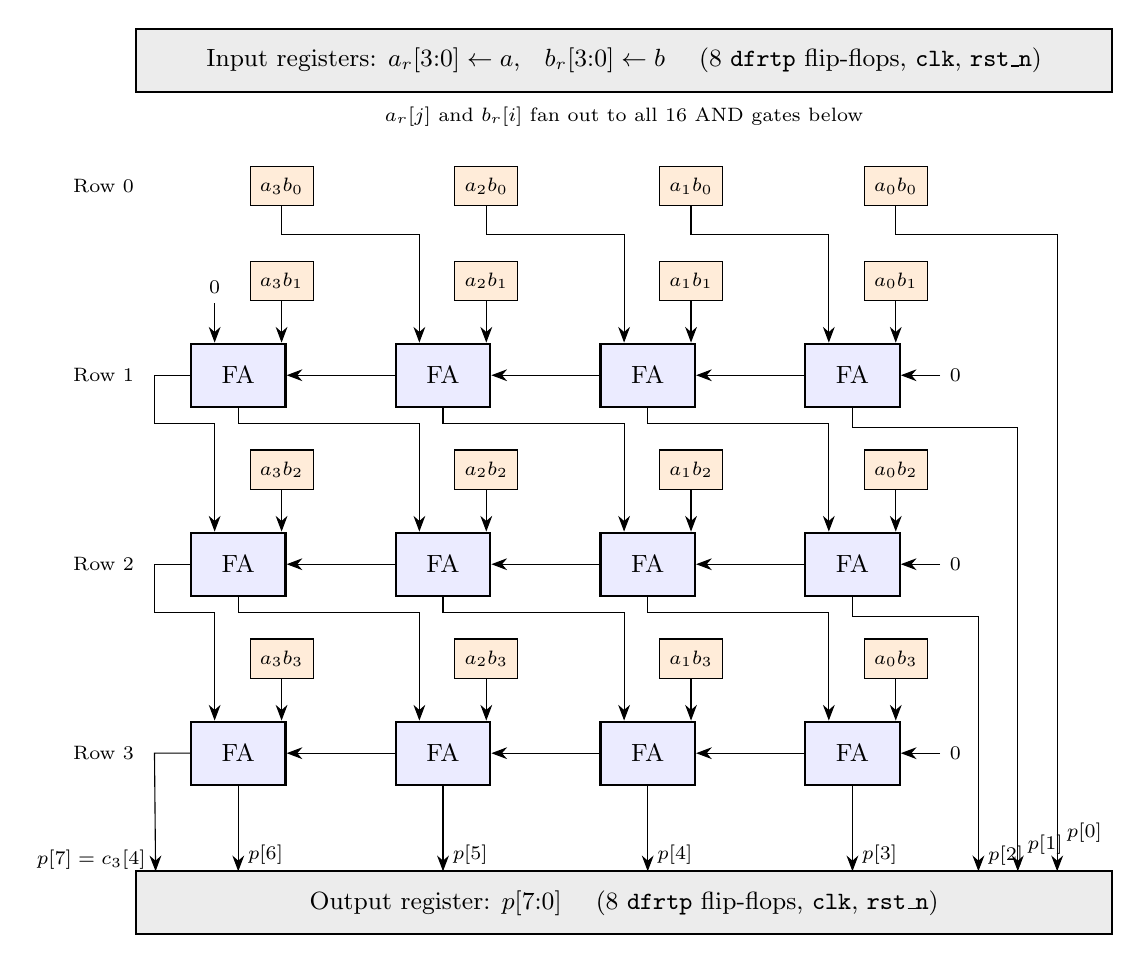
\begin{tikzpicture}[
    >={Stealth[length=2mm]},
    fa/.style={draw, thick, fill=blue!8, minimum width=12mm, minimum height=8mm, font=\small},
    andg/.style={draw, fill=orange!15, minimum width=8mm, minimum height=5mm, inner sep=1pt, font=\scriptsize},
    reg/.style={draw, thick, fill=gray!15, minimum height=8mm, font=\small, align=center},
    w/.style={->, thin},
    lbl/.style={font=\scriptsize}
]
\def\dx{2.6}
\def\dy{2.4}
% Input register
\node[reg, minimum width=124mm] (inreg) at ({1.5*\dx+1.0}, 1.6)
  {Input registers: $a_r[3{:}0] \leftarrow a$, \; $b_r[3{:}0] \leftarrow b$ \quad (8 \texttt{dfrtp} flip-flops, \texttt{clk}, \texttt{rst\_n})};
\node[lbl, anchor=north] at ($(inreg.south)+(0,-0.05)$) {$a_r[j]$ and $b_r[i]$ fan out to all 16 AND gates below};
% Row 0: AND gates only
\foreach \j in {0,...,3} {
  \pgfmathsetmacro{\x}{(3-\j)*\dx}
  \node[andg] (A0\j) at ({\x+0.55}, 0) {$a_{\j}b_{0}$};
}
\node[lbl, anchor=east] at (-1.2, 0) {Row 0};
% Rows 1-3: AND gate + full adder per column
\foreach \i in {1,2,3} {
  \pgfmathsetmacro{\y}{-\i*\dy}
  \node[lbl, anchor=east] at (-1.2, \y) {Row \i};
  \foreach \j in {0,...,3} {
    \pgfmathsetmacro{\x}{(3-\j)*\dx}
    \node[fa] (F\i\j) at (\x, \y) {FA};
    \node[andg] (A\i\j) at ({\x+0.55}, {\y+1.2}) {$a_{\j}b_{\i}$};
    \draw[w] (A\i\j.south) -- ($(F\i\j.north)+(0.55,0)$);
  }
  % carry chain, right to left
  \draw[w] ($(F\i0.east)+(0.5,0)$) node[right, lbl] {0} -- (F\i0.east);
  \foreach \j/\k in {0/1, 1/2, 2/3} {
    \draw[w] (F\i\j.west) -- (F\i\k.east);
  }
}
% Row 0 -> row 1 inputs: r0[j] = pp0[j+1], r0[3] = 0
\foreach \j/\k in {0/1, 1/2, 2/3} {
  \draw[w] (A0\k.south) -- ++(0,-0.35) -| ($(F1\j.north)+(-0.3,0)$);
}
\draw[w] ($(F13.north)+(-0.3,0.5)$) node[above, lbl] {0} -- ($(F13.north)+(-0.3,0)$);
% Rows i -> i+1: r_i[j] = s_i[j+1], r_i[3] = c_i[4]
\foreach \i/\n in {1/2, 2/3} {
  \foreach \j/\k in {0/1, 1/2, 2/3} {
    \draw[w] (F\i\k.south) -- ++(0,-0.2) -| ($(F\n\j.north)+(-0.3,0)$);
  }
  \draw[w] (F\i3.west) -- ++(-0.45,0) |- ($(F\i3.south)+(-0.3,-0.2)$) -- ($(F\n3.north)+(-0.3,0)$);
}
% Output register
\pgfmathsetmacro{\yreg}{-3*\dy-1.9}
\node[reg, minimum width=124mm] (outreg) at ({1.5*\dx+1.0}, \yreg)
  {Output register: $p[7{:}0]$ \quad (8 \texttt{dfrtp} flip-flops, \texttt{clk}, \texttt{rst\_n})};
% Product bits into the output register
\pgfmathsetmacro{\yin}{\yreg+0.4}
\draw[w] (A00.south) -- ++(0,-0.35) -| ({3*\dx+2.6}, \yin) node[pos=0.97, right, lbl] {$p[0]$};
\draw[w] (F10.south) -- ++(0,-0.25) -| ({3*\dx+2.1}, \yin) node[pos=0.97, right, lbl] {$p[1]$};
\draw[w] (F20.south) -- ++(0,-0.25) -| ({3*\dx+1.6}, \yin) node[pos=0.97, right, lbl] {$p[2]$};
\draw[w] (F30.south) -- ({3*\dx}, \yin) node[pos=0.8, right, lbl] {$p[3]$};
\draw[w] (F31.south) -- ({2*\dx}, \yin) node[pos=0.8, right, lbl] {$p[4]$};
\draw[w] (F32.south) -- ({1*\dx}, \yin) node[pos=0.8, right, lbl] {$p[5]$};
\draw[w] (F33.south) -- ({0*\dx}, \yin) node[pos=0.8, right, lbl] {$p[6]$};
\draw[w] (F33.west) -- ++(-0.45,0) -- ({-0.45-0.6}, \yin) node[pos=0.9, left, lbl] {$p[7] = c_3[4]$};
\end{tikzpicture}}
\caption{Block diagram of \texttt{mult\_array}: 16 AND gates ($a_j b_i = pp_i[j]$), 12 full adders in
three ripple-carry rows, and the input and output registers (16 flip-flops). Each full adder takes
$pp_i[j]$ on its right input and $r_{i-1}[j]$ on its left input; carries ripple from right to left.}
\label{fig:block}
\end{figure*}

\begin{figure*}[!t]
\centering
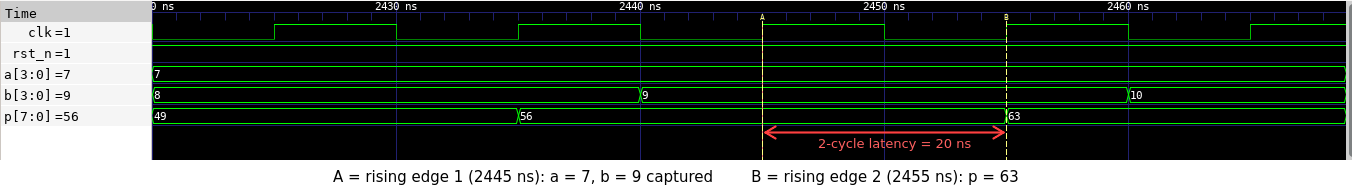
\includegraphics[width=\textwidth]{images/waveform_7x9.png}
\caption{GTKWave view of \texttt{clk}, \texttt{rst\_n}, $a$, $b$ and $p$ (decimal) for the example
$7 \times 9$. Markers A and B are the two rising edges of the 2-cycle latency.}
\label{fig:wave}
\end{figure*}

% ---------------------------------------------------------------------------
\section{Part A: RTL Design and Verification}

\subsection{Testbench}
\cell{tb_mult} generates a \SI{10}{\nano\second} clock, holds \texttt{rst\_n} low for the first
two cycles and then applies all 256 combinations of $a$ and $b$. Inputs change on the falling edge.
After two rising edges the testbench waits another half cycle and compares $p$ with $a \times b$
(the \texttt{*} operator is used only here). The comparison uses \texttt{!==}, so an unknown output
also counts as an error. The testbench prints a line for every mismatch and one summary line, and
writes \texttt{mult.vcd}. The RTL result is:
\begin{center}\small\texttt{PASS: 256 vectors checked, 0 errors}\end{center}

\subsection{Error-detection check}
We temporarily changed the sum in \cell{full_adder.v} to \texttt{a \^{} b}, which ignores the carry
input. The same testbench then reports 95 mismatches, the first being $a = 3$, $b = 3$, $p = 5$
(expected 9):
\begin{center}\small\texttt{FAIL: 256 vectors checked, 95 errors}\end{center}
The change was then undone, and the testbench passes again.

\subsection{Hand-worked example}
We used Sudhanva Joshi's roll number (2023102022). Its last digit is 2, so $A = 2 + 5 = 7$, and
because $A = 7$ the assignment gives $B = 9$.
\begin{center}
\small
\begin{tabular}{r@{\hspace{3pt}}c@{\hspace{3pt}}c@{\hspace{3pt}}c@{\hspace{3pt}}c@{\hspace{3pt}}c@{\hspace{3pt}}c@{\hspace{3pt}}c@{\hspace{3pt}}c@{\hspace{8pt}}l}
 & & & & & 0 & 1 & 1 & 1 & $A = 7$ \\
 $\times$ & & & & & 1 & 0 & 0 & 1 & $B = 9$ \\ \cmidrule{2-9}
 & & & & & 0 & 1 & 1 & 1 & $pp_0$ ($b_0 = 1$) \\
 & & & & 0 & 0 & 0 & 0 & & $pp_1$ ($b_1 = 0$), shift 1 \\
 & & & 0 & 0 & 0 & 0 & & & $pp_2$ ($b_2 = 0$), shift 2 \\
 & & 0 & 1 & 1 & 1 & & & & $pp_3$ ($b_3 = 1$), shift 3 \\ \cmidrule{2-9}
 & 0 & 0 & 1 & 1 & 1 & 1 & 1 & 1 & $P = 63$ \\
\end{tabular}
\end{center}
In the array, $r_0 = 0011$.
\begin{itemize}
\item Row~1 adds $pp_1 = 0000$: $s_1 = 0011$, so $p[1] = 1$ and $r_1 = 0001$.
\item Row~2 adds $pp_2 = 0000$: $s_2 = 0001$, so $p[2] = 1$ and $r_2 = 0000$.
\item Row~3 adds $pp_3 = 0111$: $s_3 = 0111$ and $c_3[4] = 0$, so $p[3] = 1$ and
$p[7{:}4] = 0011$.
\end{itemize}
Hence $P = 0011\,1111_2 = 63$.

\subsection{Waveform}
Fig.~\ref{fig:wave} shows the example in the RTL simulation. With $a = 7$ throughout, $b$ changes
from 8 to 9 on the falling edge at \SI{2440}{\nano\second}. Rising edge~1 at
\SI{2445}{\nano\second} (marker~A) captures $a$ and $b$ into the input registers. Rising edge~2 at
\SI{2455}{\nano\second} (marker~B) captures the product, and $p$ changes from 56 to 63. The latency
is two clock cycles, or \SI{20}{\nano\second}.

% ---------------------------------------------------------------------------
\section{Part B: Logic Synthesis}

The Yosys script \cell{synth/synth.tcl} performs these steps:
\begin{enumerate}
\item read both RTL files;
\item run generic synthesis with the full adders flattened into one module;
\item map the flip-flops, and then the logic (with ABC), to the typical-corner Liberty library;
\item remove unused wires;
\item write the cell and area report and the gate-level netlist.
\end{enumerate}
Table~\ref{tab:synth} summarises the results. All cell names omit the library prefix
\cell{sky130_fd_sc_hd__}. The flip-flop cell \cell{dfrtp_1} has an area of
\SI{25.024}{\square\micro\metre}.

\begin{table}[!t]
\centering
\caption{Part B results}
\label{tab:synth}
\small
\begin{tabular}{@{}lr@{}}
\toprule
Metric & Value \\
\midrule
Total number of cells & 61 \\
Number of flip-flops & 16 \\
Total cell area & \SI{756.976}{\square\micro\metre} \\
Flip-flop area ($16 \times 25.024$) & \SI{400.384}{\square\micro\metre} \\
Flip-flop area (share of total) & \SI{52.89}{\percent} \\
\midrule
\multicolumn{2}{@{}l}{Three most-used cell types} \\
\quad \cell{dfrtp_1} & 16 \\
\quad \cell{nand2_1} & 7 \\
\quad \cell{maj3_1} and \cell{and2_0} (tied) & 4 each \\
\midrule
\multicolumn{2}{@{}l}{Netlist simulation} \\
\multicolumn{2}{@{}r@{}}{\small\texttt{PASS: 256 vectors checked, 0 errors}} \\
\bottomrule
\end{tabular}
\end{table}

We simulated the gate-level netlist against the SKY130 functional cell models with unit gate
delays, using the same testbench. It passes all 256 vectors, so synthesis preserved the behaviour.
The netlist also contains two \cell{lpflow_isobufsrc_1} cells. ABC is free to pick them because
the script does not exclude any library cells.

% ---------------------------------------------------------------------------
\section{Part C: Static Timing Analysis}

The OpenSTA script \cell{sta/sta.tcl} reads the typical-corner library and the netlist. It then
defines the clock, sets \SI{1.0}{\nano\second} input and output delays, and reports the worst setup
slack and the critical path. At $T = \SI{10}{\nano\second}$ the worst slack is
\SI{7.213}{\nano\second}, so
\begin{align*}
\Tmin &= 10 - 7.213 = \SI{2.787}{\nano\second} \approx \SI{2.79}{\nano\second},\\
\Fmax &= 1000 / 2.79 = \SI{358.4}{\mega\hertz}.
\end{align*}
Rerunning at $T = \SI{2.79}{\nano\second}$ gives \SI{0.003}{\nano\second} of slack
(Table~\ref{tab:sta}).

\begin{table}[!t]
\centering
\caption{Part C results (typical corner)}
\label{tab:sta}
\small
\begin{tabular}{@{}lr@{}}
\toprule
Metric & Value \\
\midrule
Worst slack at $T = \SI{10}{\nano\second}$ & \SI{7.213}{\nano\second} \\
$\Tmin$ & \SI{2.79}{\nano\second} \\
$\Fmax$ & \SI{358.4}{\mega\hertz} \\
Slack at $T = \Tmin$ & \SI{0.003}{\nano\second} \\
Critical path start point & \cell{_91_} ($a_r[1]$) \\
Critical path end point & \cell{_88_} ($p[6]$) \\
Cells on the critical path & 9 logic, 2 flip-flops \\
Latency ($2 \times \Tmin$) & \SI{5.58}{\nano\second} \\
Throughput & \num{358.4} million results/s \\
\bottomrule
\end{tabular}
\end{table}

The critical path (Table~\ref{tab:path}) runs from the register holding $a_r[1]$ to the register
that captures $p[6]$. Five of its nine logic cells are recognisable full-adder cells: three
\cell{maj3} cells (carry) and the \cell{xnor3} and \cell{xor3} cells (sum). The first three cells
implement the partial products and the simplified first adder row, which ABC merged into complex
gates.

\begin{table}[!t]
\centering
\caption{Critical path at $T = \SI{2.79}{\nano\second}$}
\label{tab:path}
\small
\begin{tabular}{@{}rllr@{}}
\toprule
\# & Cell & Role & Delay (\si{\nano\second}) \\
\midrule
-- & \cell{dfrtp_1} (\cell{_91_}) & launch, clock to Q & 0.398 \\
1 & \cell{clkinv_1} & partial products & 0.073 \\
2 & \cell{o311ai_0} & partial products, row 1 & 0.356 \\
3 & \cell{a21oi_1} & row 1 & 0.153 \\
4 & \cell{maj3_1} & FA carry & 0.402 \\
5 & \cell{xnor3_1} & FA sum & 0.370 \\
6 & \cell{maj3_1} & FA carry & 0.368 \\
7 & \cell{maj3_1} & FA carry & 0.354 \\
8 & \cell{xor3_1} & FA sum & 0.178 \\
-- & \cell{dfrtp_1} (\cell{_88_}) & capture, setup time & 0.135 \\
\midrule
 & \multicolumn{2}{l}{Data arrival time} & 2.652 \\
\bottomrule
\end{tabular}
\end{table}

% ---------------------------------------------------------------------------
\section{Part D: Physical Design}

\subsection{Configuration}
Table~\ref{tab:config} lists the settings in \cell{pnr/config.json}. The clock period is
$1.2 \times \Tmin = 1.2 \times 2.79 = \SI{3.348}{\nano\second}$, rounded up to the next
\SI{0.5}{\nano\second}. As in Part~C, timing is signed off at the typical corner only, which the
\cell{STA_CORNERS} setting selects.

\begin{table}[!t]
\centering
\caption{LibreLane configuration}
\label{tab:config}
\small
\begin{tabular}{@{}ll@{}}
\toprule
Key & Value \\
\midrule
\cell{DESIGN_NAME} & \cell{mult_array} \\
\cell{VERILOG_FILES} & \cell{full_adder.v}, \cell{mult_array.v} \\
\cell{CLOCK_PORT} & \cell{clk} \\
\cell{CLOCK_PERIOD} & \SI{3.5}{\nano\second} \\
\cell{FP_SIZING} & \cell{absolute} \\
\cell{DIE_AREA} & $0, 0, 150, 150$ (\si{\micro\metre}) \\
\cell{STA_CORNERS} & \cell{nom_tt_025C_1v80} \\
\bottomrule
\end{tabular}
\end{table}

\subsection{Results}
The flow finished in a single run at \SI{3.5}{\nano\second} with positive setup slack, 0 DRC errors
and 0 LVS errors. Table~\ref{tab:pnr} lists the final metrics from \cell{pnr/metrics.json}. The
post-route maximum frequency is
\[
\Fmax = \frac{1000}{3.5 - 0.077} = \frac{1000}{3.423} = \SI{292.2}{\mega\hertz},
\]
\SI{18}{\percent} lower than the \SI{358.4}{\mega\hertz} from Part~C. The post-route critical path
runs from the $a_r[0]$ register to the $p[6]$ register through eight logic cells. Four of them are
full-adder cells: \cell{xor3}, two \cell{maj3} and \cell{xnor3}.

\begin{table}[!t]
\centering
\caption{Part D results (typical corner)}
\label{tab:pnr}
\small
\begin{tabular}{@{}lr@{}}
\toprule
Metric & Value \\
\midrule
\cell{CLOCK_PERIOD} used & \SI{3.5}{\nano\second} \\
Number of runs needed & 1 \\
Core area & \SI{17759.5}{\square\micro\metre} \\
Die area & \SI{22500}{\square\micro\metre} \\
Cells after synthesis (Part B) & 61 \\
Cells after place and route & 1882 \\
Kinds of cells added & decap, fill, tap, buffers \\
Wirelength & \SI{2495}{\micro\metre} \\
Setup slack & \SI{0.077}{\nano\second} \\
Post-route $\Fmax$ & \SI{292.2}{\mega\hertz} \\
$\Fmax$ from Part C & \SI{358.4}{\mega\hertz} \\
DRC errors (Magic, KLayout) & 0, 0 \\
LVS errors & 0 \\
\bottomrule
\end{tabular}
\end{table}

\subsection{Cells added by the flow}
Table~\ref{tab:cells} breaks down the 1882 instances. LibreLane re-synthesises the RTL itself and
produces 62 logic and flip-flop cells. That is one more than Part~B, because LibreLane's synthesis
does not use the \cell{lpflow} cells. Every other cell was added during physical design.

\begin{table}[!t]
\centering
\caption{Cells after place and route}
\label{tab:cells}
\small
\begin{tabular}{@{}lr@{}}
\toprule
Cell kind & Count \\
\midrule
Design logic and flip-flops & 62 \\
Decap (\cell{decap_3} to \cell{decap_12}) & 1300 \\
Fill (\cell{fill_1}, \cell{fill_2}) & 253 \\
Well taps (\cell{tapvpwrvgnd_1}) & 245 \\
Timing-repair buffers (\cell{buf_2}, \cell{clkdlybuf4s50_1}) & 19 \\
Clock-tree buffers (\cell{clkbuf_16}) & 3 \\
\midrule
Total & 1882 \\
\bottomrule
\end{tabular}
\end{table}

\subsection{Layout}
Fig.~\ref{fig:layout} shows the final GDS in KLayout.
\begin{itemize}
\item \textbf{Whole die:} the \SI{150}{\micro\metre} die, the standard-cell rows and the I/O pins on
the die edges. The signal routing is concentrated in the middle of the core, where the 78 logic,
flip-flop and buffer cells sit; the rest of the rows hold decap and fill cells.
\item \textbf{Zoomed view:} the rows bounded by horizontal power rails, the poly gates inside the
cells, horizontal metal~1 and vertical metal~2 wires, and the vias between them.
\end{itemize}

\begin{figure*}[!t]
\centering
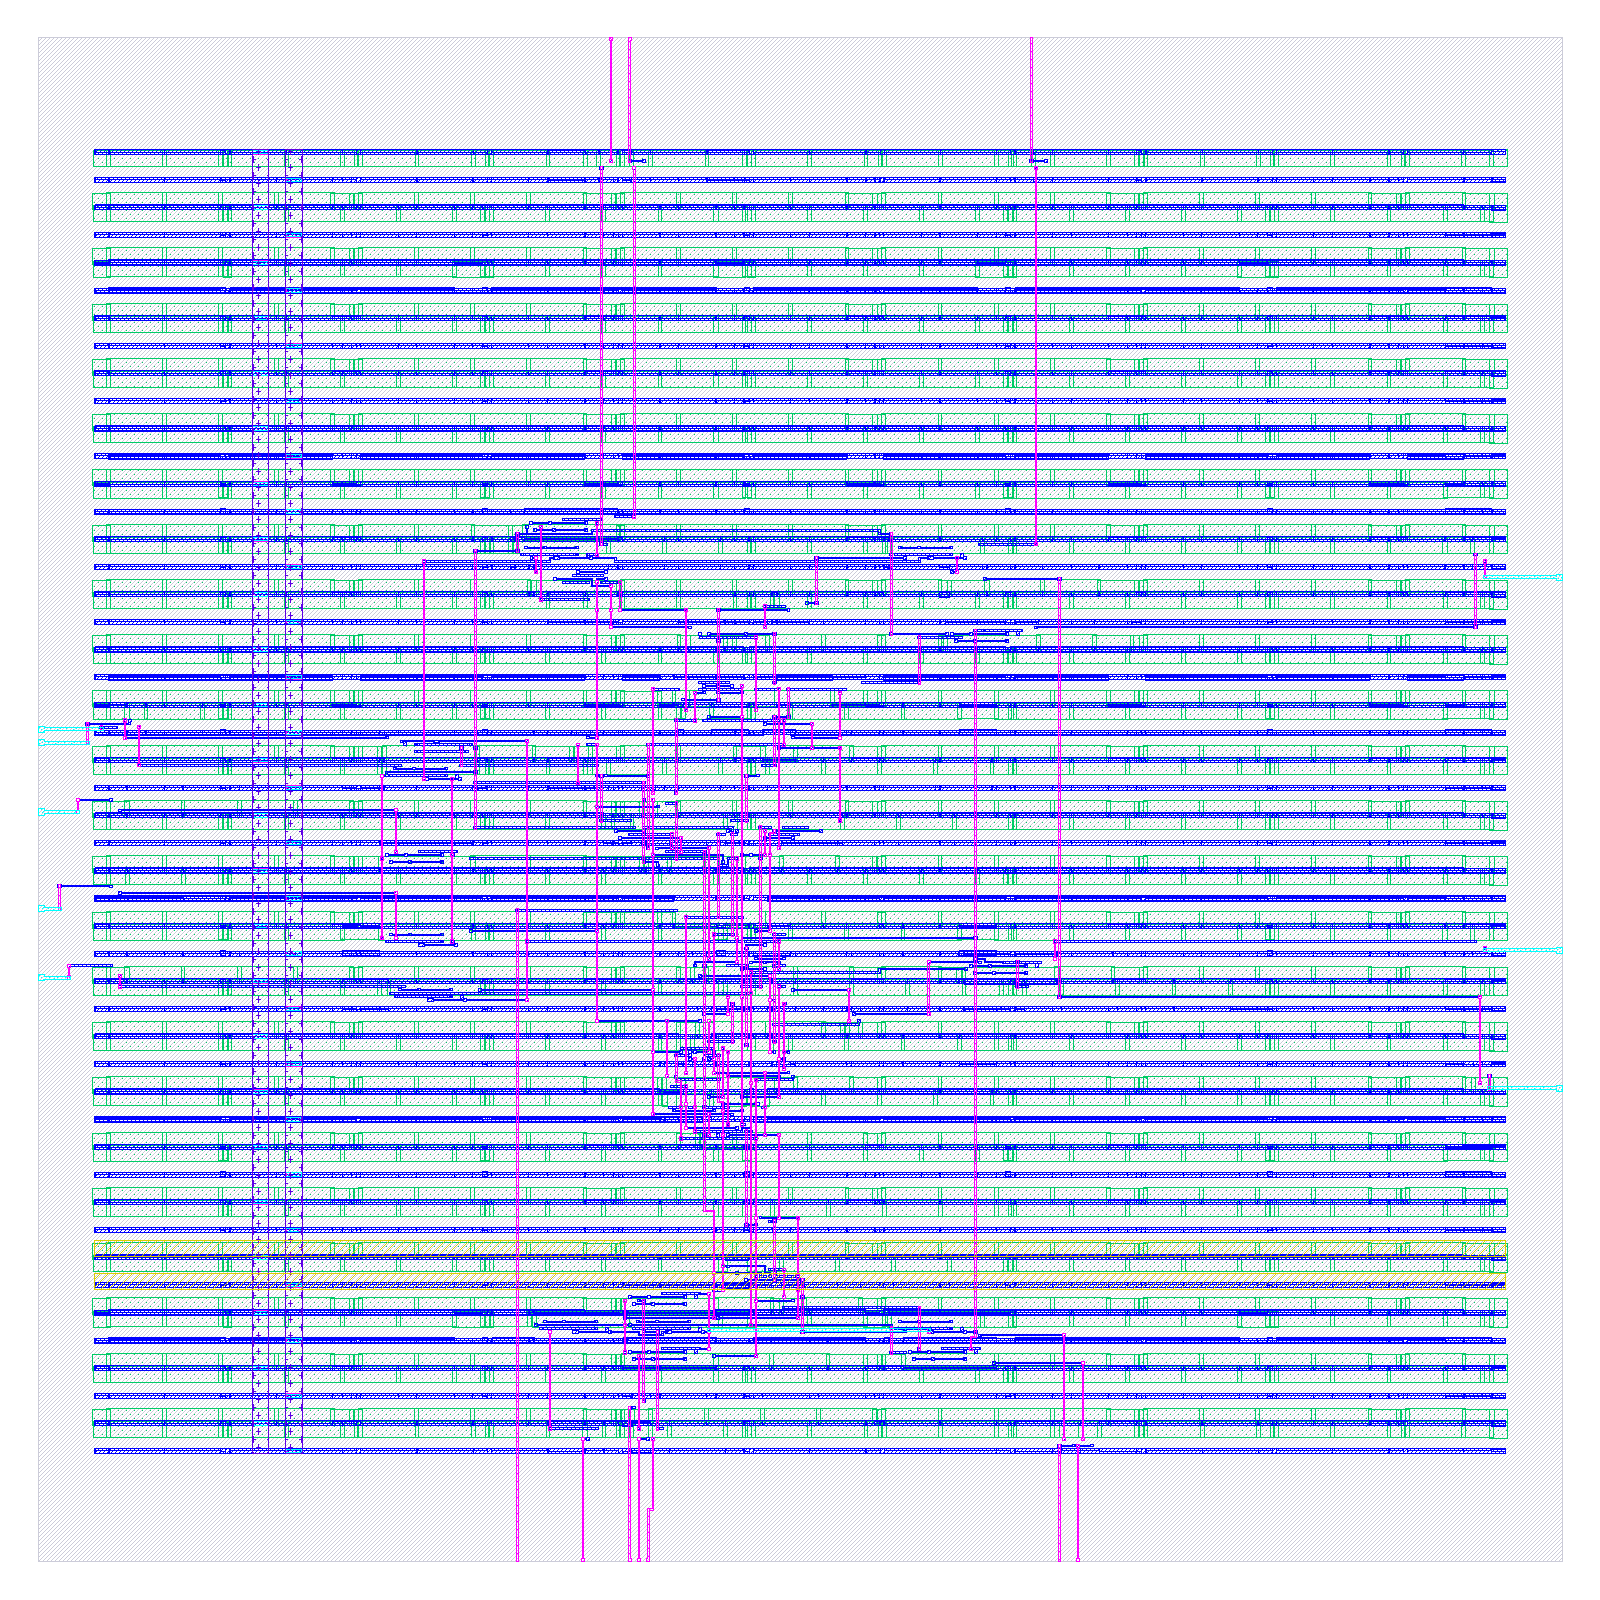
\includegraphics[width=0.48\textwidth]{images/layout_die.png}\hfill
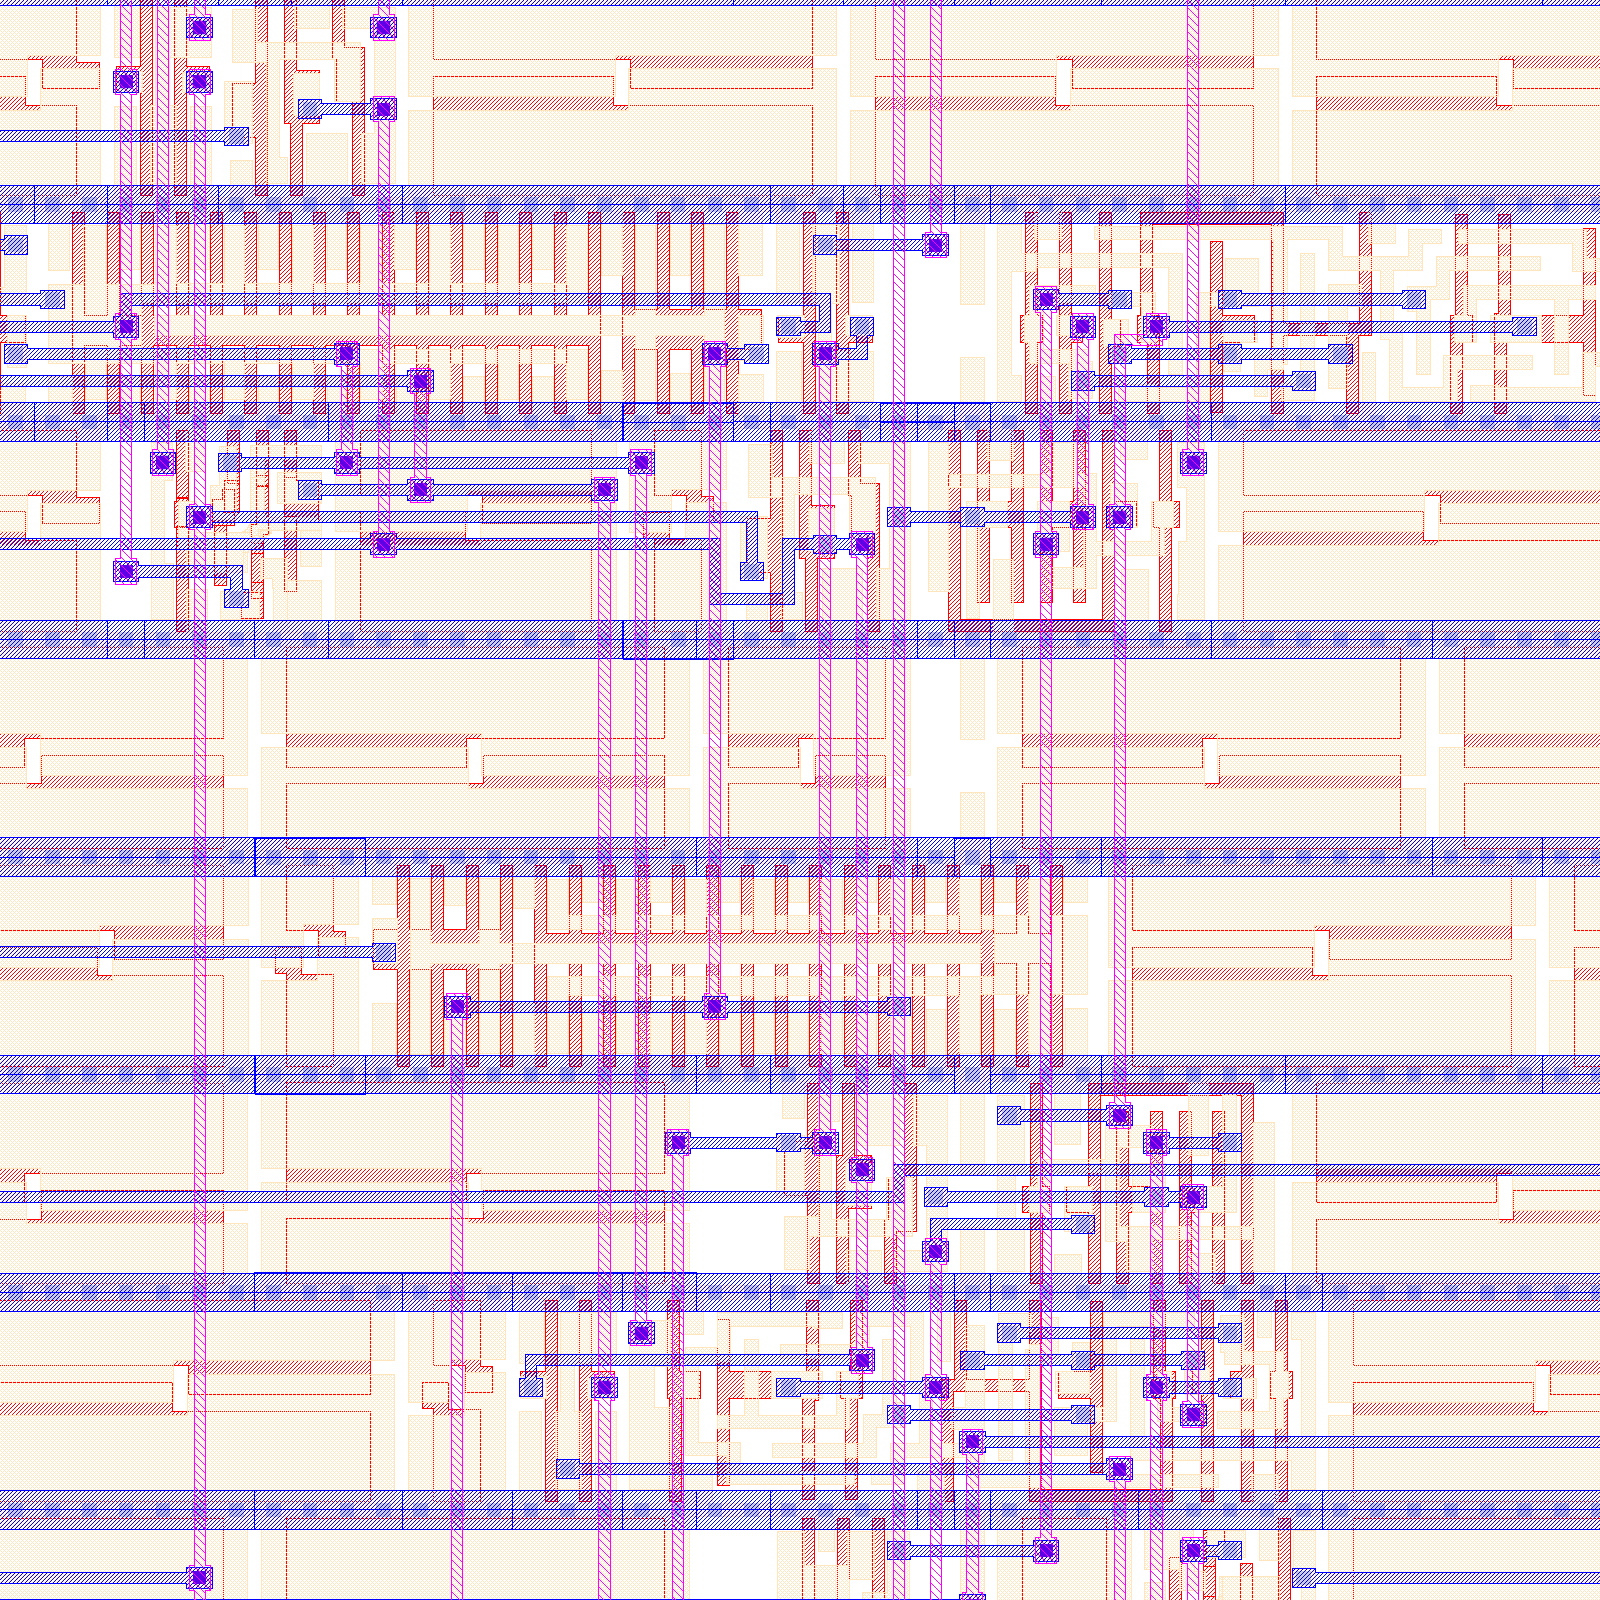
\includegraphics[width=0.48\textwidth]{images/layout_zoom.png}
\caption{Final layout in KLayout. Left: whole die (\qtyproduct{150 x 150}{\micro\metre};
metal layers, n-well and boundary). Right: zoomed view of about
\qtyproduct{20 x 20}{\micro\metre} (poly, local interconnect, metal~1, metal~2 and vias).}
\label{fig:layout}
\end{figure*}

\subsection{A note on process corners}
By default LibreLane signs off at nine process corners. Before we restricted signoff to the
typical corner, exploratory runs with all corners met timing at the typical corner. They failed
only at the slow corner (\SI{100}{\celsius}, \SI{1.60}{\volt}), where the path is roughly twice as
slow. The README records these runs. The assignment evaluates timing at the typical corner, so the
reported run uses that corner only.

% ---------------------------------------------------------------------------
\section{Answers to the Questions}

\textbf{Q1.} Synthesis produced $61 - 16 = 45$ logic cells for the array, instead of
$16 + 12 = 28$ blocks. The count is not one cell per block, because flattening dissolves the
full-adder boundaries and ABC re-optimises the whole logic cone. Some effects add cells:
\begin{itemize}
\item Some full adders are split into a sum cell (\cell{xor3}, \cell{xnor3} or \cell{xor2}) and a
carry cell (\cell{maj3}), or into several smaller gates.
\item The library's full-adder cell \cell{fa_1} has two outputs, which ABC cannot map to; it reports
it as a multi-output cell and skips it. Each full adder therefore costs at least two cells.
\end{itemize}
Others remove cells:
\begin{itemize}
\item Adders with a constant-0 input ($c_i[0] = 0$, $r_0[3] = 0$) reduce to half adders.
\item AND gates are merged into complex cells such as \cell{a21oi}, \cell{a22oi} and
\cell{o311ai}.
\end{itemize}

\textbf{Q2.} At $\Tmin = \SI{2.79}{\nano\second}$, the critical path runs from the input-register
flip-flop holding $a_r[1]$ to the output-register flip-flop that captures $p[6]$. It has nine logic
cells between the two flip-flops (Table~\ref{tab:path}), five of them full-adder cells. The estimate
of $2N = 8$ full-adder delays describes the unoptimised array. Here the first stages are simplified
into three fast complex gates (half adders and merged AND logic), so only five full-adder stages
remain. Those five cells take \SI{1.672}{\nano\second}, about \SI{0.33}{\nano\second} each, and the
three first-stage gates take \SI{0.582}{\nano\second}. The total logic delay of
\SI{2.254}{\nano\second} therefore corresponds to about seven full-adder delays, slightly below the
estimate of eight.

\textbf{Q3.} Flip-flops take \SI{52.89}{\percent} of the total cell area: 400.384 of
\SI{756.976}{\square\micro\metre}. A \cell{dfrtp_1} with asynchronous reset is
\SI{25.0}{\square\micro\metre}, about seven times a \cell{nand2_1} (\SI{3.75}{\square\micro\metre}),
because it contains two latches, a clock inverter and reset logic. The design needs 16 of them
(8 input bits and 8 output bits), while the combinational array is only 45 small gates. The number
of registers grows linearly with $N$, but the array grows with $N^2$, so the flip-flop share is
largest for small multipliers.

\textbf{Q4.} The post-route $\Fmax$ is \SI{292.2}{\mega\hertz}, against \SI{358.4}{\mega\hertz} in
Part~C. Three effects lower it:
\begin{itemize}
\item The routed wires add resistance and capacitance, which are extracted after routing.
\item The flow adds a \SI{0.25}{\nano\second} clock uncertainty and a \SI{5}{\percent} timing
derate.
\item The inputs are driven by a real cell and the outputs drive a real load.
\end{itemize}
Together these stretch the launch-to-capture data path from \SI{2.652}{\nano\second} to
\SI{3.03}{\nano\second}. The flow added five kinds of cells (Table~\ref{tab:cells}), each for a
reason:
\begin{itemize}
\item \textbf{Clock-tree buffers} (\cell{clkbuf_16}) deliver the clock to all 16 flip-flops with
low skew. They add \SI{0.32}{\nano\second} of insertion delay, which is common to the launch and
capture flip-flops.
\item \textbf{Timing-repair buffers} fix slew and capacitance limits and improve timing.
\item \textbf{Tap cells} tie the n-wells and the substrate to VPWR and VGND, preventing latch-up.
\item \textbf{Decap cells} add capacitance between the supply rails, reducing supply noise when
cells switch.
\item \textbf{Fill cells} close the remaining gaps in the rows, so that the wells, implants and
power rails are continuous, as the design rules require.
\end{itemize}

\textbf{Q5.} A DRC (design rule check) verifies that the layout geometry obeys the foundry's
manufacturing rules: minimum widths, spacings, enclosures, overlaps and densities on every layer.
An LVS (layout versus schematic) check extracts the transistors and their connections from the
layout and compares them with the netlist. It confirms that the layout implements exactly the
intended circuit, with no shorts, opens or missing devices. Both must pass before fabrication:
\begin{itemize}
\item A DRC violation can make the chip impossible to manufacture reliably, for example through
shorts, broken wires or low yield.
\item An LVS mismatch gives a chip that can be manufactured but does the wrong thing.
\end{itemize}
Our final layout has 0 DRC errors (Magic and KLayout) and 0 LVS errors (Netgen).

\textbf{Q6.} For an 8-bit multiplier ($N = 8$):
\begin{itemize}
\item \textbf{Size:} the array needs $N^2 = 64$ AND gates and \mbox{$N(N-1) = 56$} full adders, against 16
and 12 for $N = 4$. That is about 4.7 times as many full adders, so the logic area grows roughly
with $N^2$.
\item \textbf{Path length:} the critical path is about $2N = 16$ full-adder delays instead of 8,
twice as long. The delay grows linearly with $N$.
\item \textbf{Delay estimate:} in Part~C, the 4-bit logic delay is
\mbox{$2.652 - 0.398 = \SI{2.254}{\nano\second}$}. Scaling it by $16/8$ gives about
\SI{4.5}{\nano\second} of logic. Adding the clock-to-Q time (\SI{0.40}{\nano\second}) and the
setup time (\SI{0.14}{\nano\second}) gives $\Tmin \approx \SI{5.0}{\nano\second}$, or
$\Fmax \approx \SI{200}{\mega\hertz}$, against \SI{358}{\mega\hertz} for the 4-bit design.
\item \textbf{Registers:} the design would need $8 + 8 + 16 = 32$ flip-flops.
\end{itemize}

% ---------------------------------------------------------------------------
\section{Conclusion}
We took the 4-bit array multiplier from RTL to a DRC- and LVS-clean SKY130 layout. It is
functionally correct in both RTL and gate-level simulation. At the typical corner it runs at
\SI{358}{\mega\hertz} before layout and \SI{292}{\mega\hertz} after routing, on a
\qtyproduct{150 x 150}{\micro\metre} die. All source files, scripts and generated reports are in
the repository at \url{https://github.com/SudhuJ/arrayMultiplier}, whose README lists every
command, in order.

\end{document}
